\begin{figure*}[t]
  \centering
  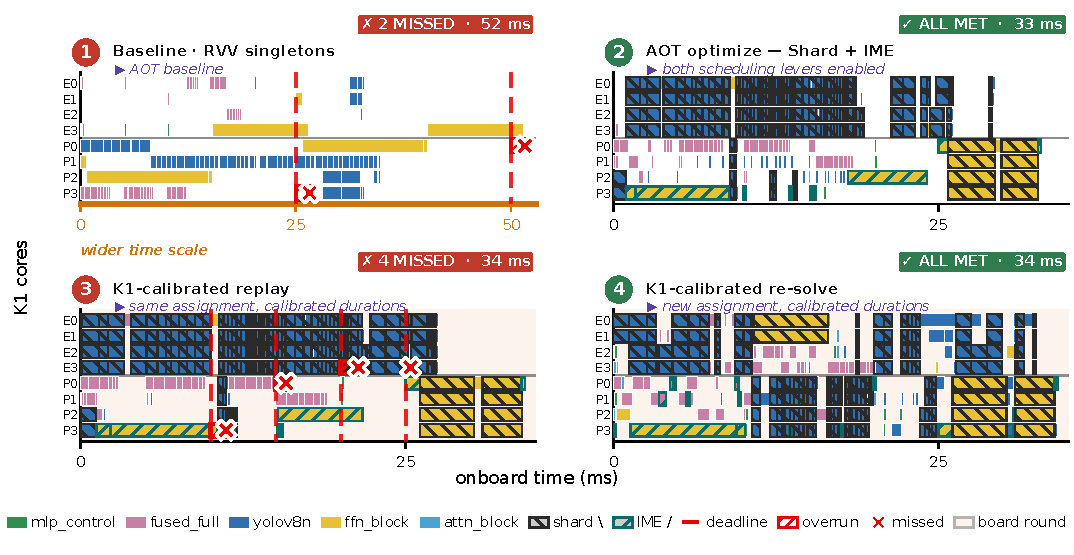
\includegraphics[width=\textwidth]{results/codesign_feedback/schedule_evolution_mega.pdf}
  \caption{Four-stage scheduling feedback loop for the contended sensor-fusion
  workload. (1) The RVV singleton baseline misses two FFN instance deadlines.
  (2) Ahead-of-time sharding and IME routing reduce the modeled makespan from
  51.61 to 32.85\,ms and meet every instance deadline. (3) Re-timing that fixed
  assignment with K1 calibration (per-dispatch/per-operation measurements where
  available and aggregate fallback otherwise) exposes four misses (two
  navigation, one control, and one FFN) at 34.16\,ms. (4) CP-SAT re-solves
  with the same calibrated costs and recovers every deadline at 34.16\,ms.
  Red dashed lines mark deadlines, hatched extensions mark overruns, and
  crosses mark late instance completions. The calibrated panels are schedule
  models grounded in K1 measurements, not direct execution traces.}
  \label{fig:schedule-feedback-loop}
\end{figure*}
